\documentclass[a4paper,landscape,8pt,fleqn]{scrartcl}
\usepackage[english]{babel}
\usepackage[utf8]{inputenc}
\usepackage[a4paper, landscape, margin=1.1cm]{geometry}
\usepackage{latexsym}
\usepackage{multicol}
\usepackage{amsmath}
\usepackage{amsfonts}
\usepackage{amssymb}
\usepackage{array}
\usepackage{graphicx}
\usepackage{booktabs}
\usepackage{empheq}			% emphasize (box) equations
\usepackage{float}				% add H as an option for floats
\usepackage{parskip}			% add no indentation to new paragraphs
\usepackage{enumitem}		% description lists
\usepackage{fancyhdr}
\usepackage{lastpage}
\usepackage{framed}

\pagestyle{plain}
\columnsep 30pt
\columnseprule .4pt

\setlength{\mathindent}{0.1cm}

\newcommand*\widefbox[1]{\fbox{\hspace{1em}#1\hspace{1em}}}		% required for boxing several lines of equations at once

\renewcommand*{\familydefault}{\sfdefault}		% set font to default sans-serif

\renewcommand{\labelitemi}{\tiny$\blacksquare$}		% change symbol of itemized lists
\setlist[itemize]{leftmargin=0.4cm}								% reduce indentation of itemized lists
\renewcommand{\labelenumi}{(\roman{enumi})}			% change counter of enumerated lists
\setlist[enumerate]{leftmargin=0.4cm}							% reduce indentation of enumerated lists

\renewcommand{\arraystretch}{1}
\renewcommand{\emph}[1]{\textbf{#1}}

\graphicspath{ {images/} }

\pagestyle{fancy}
\fancyhead{}
\setlength{\headheight}{0pt}
\setlength{\footheight}{14pt}
\renewcommand{\headrulewidth}{0pt}
\renewcommand{\footrulewidth}{0.5pt}
\lfoot{Fabian MARBACH}
\cfoot{p \thepage\ / \pageref{LastPage}}
\rfoot{New Trends in Stochastic Portfolio Theory}

%\allowdisplaybreaks	% equations can be split on two pages/columns

\usepackage{parskip}	% add no indentation to new paragraphs

\makeatletter
\renewcommand{\section}{\@startsection{section}{1}{0mm}%
{-2\baselineskip}{0.8\baselineskip}%
{\hrule depth 0.2pt width\columnwidth\hrule depth1.5pt
width0.25\columnwidth\vspace*{1.2em}\Large\bfseries}}
\makeatother

\makeatletter
\renewcommand{\subsection}{\@startsection{subsection}{1}{0mm}%
{-2\baselineskip}{0.8\baselineskip}%
{\hrule depth 0.2pt width\columnwidth\hrule depth0.75pt
width0.25\columnwidth\vspace*{1.2em}\large\bfseries}}
\makeatother

\makeatletter
\renewcommand{\subsubsection}{\@startsection{subsubsection}{1}{0mm}%
{-2\baselineskip}{0.8\baselineskip}%
{\hrule depth 0.2pt width\columnwidth\vspace*{1.2em}\normalsize\bfseries}}
\makeatother

\newcommand{\Mx}[1]{\begin{bmatrix}#1\end{bmatrix}}
\newcommand{\dd}[2]{\frac{\text{d}#1}{\text{d}#2}}
\newcommand{\DD}[2]{\frac{\text{D}#1}{\text{D}#2}}
\newcommand{\deidei}[2]{\frac{\partial#1}{\partial#2}}
\newcommand{\Lbrace}[1]{\left\{\begin{array}{ll}#1\end{array}\right.} % left brace with text

% Declare mathematical operators
\DeclareMathOperator{\erf}{erf}					% error function
\DeclareMathOperator{\Var}{Var}				% variance
\DeclareMathOperator{\Varn}{Varn}			% variation
\DeclareMathOperator{\QV}{QV}				% quadratic variation
\DeclareMathOperator{\Cov}{Cov}				% covariance
\DeclareMathOperator{\Ber}{Ber}				% Bernoulli distribution
\DeclareMathOperator{\Bin}{Bin}				% Binomial distribution
\DeclareMathOperator{\Geom}{Geom}		% Geometric distribution
\DeclareMathOperator{\Poi}{Poi}					% Poisson distribution
\DeclareMathOperator{\Gammaa}{Gamma}	% Gamma distribution
\DeclareMathOperator{\Cau}{Cau}				% Cauchy distribution
\DeclareMathOperator{\Adj}{Adj}				% Adjoint
\DeclareMathOperator{\Bias}{Bias}				% Bias of an estimator
\DeclareMathOperator{\rank}{rank}				% rank
\DeclareMathOperator{\sgn}{sgn}				% signum

\begin{document}
\part*{Summary: New Trends in Stochastic Portfolio Theory}
Fabian MARBACH, Autumn Semester 2015/16
\begin{multicols*}{3}
%\tableofcontents
%\end{multicols}
%{\vspace*{0.3cm}}
%{\hrule depth 0.2pt}
%{\vspace*{0.3cm}}
%\begin{multicols}{2}
\raggedcolumns
\newpage

\section{Basics of Stochastic Portfolio Theory}

\subsection{Introduction}

\begin{itemize}
\item SPT is \emph{descriptive} as opposed to normative.
\item SPT is \emph{consistent with observable characteristics} of actual portfolios and markets.
\item As a theoretical tool, SPT offers fresh \emph{insights into equity market structure and arbitrage}.
\item SPT has been the \emph{basis of successful investment strategies} for over a decade.
\item SPT, in contrast to the classical portfolio theory of Harry Markowitz (1952), is \emph{appliable under a wide range of assumptions and conditions} that may hold in actual equity markets. \\
Unlike dynamic asset pricing, it is consistent with either equilibrium or disequilibrium, with either arbitrage or no-arbitrage, and is not predicated to the existance of EMM(s).
\item While SPT has been developed with equity markets in mind, a reasonable portion of the theory is \emph{valid for general financial assets}, as long as the asset values remain positive.
\end{itemize}

\subsection{Underlying assumptions}

\begin{itemize}
\item Probability space: $\left( \Omega,\mathcal{F},\mathbb{P} \right)$
\item The \emph{number of companies} in the market is \emph{finite and fixed}.
\item The \emph{total number of shares of each company is constant}.
\item Companies \emph{do not merge or break up}.
\item Trading is continuous in time, with \emph{no transaction costs or taxes}.
\item Shares are infinitely divisible and thus w.l.o.g., it is assumed that \emph{each company has a single share outstanding}.
\item Dividends are paid continuously rather than discretely, but in general it is assumed that there are \emph{no dividends}.
\item There is \emph{no riskless asset} included in the model, since the purpose of SPT is to study the behaviour of stock portfolios, for which the existence of a riskless asset is irrelevant.
\end{itemize}

\subsection{Stock price process}

\paragraph{Logarithmic model for the stock price processes}

\begin{align*}
d\log X_i(t) &= \underbrace{\gamma_i(t) dt}\limits_\text{bounded variation comp.} + \underbrace{\sum_{\nu=1}^n \xi_{i \nu}(t) dW_\nu(t)}\limits_\text{local mart. comp.} \\
\log X_i(t) &= \underbrace{\log X_0^i}\limits_\text{initial value} + \int_0^t \gamma_i(s) ds + \int_0^t \sum_{\nu=1}^n \xi_{i \nu}(s) dW_\nu(s)
\end{align*}
Remarks:
\begin{itemize}
\item Time: $t,T \in [0,\infty)$
\item \emph{Stock price processes} $X_i(t) > 0, \quad \forall t \in [0, \infty)$:
\begin{itemize}
\item $X_i$ represent stock prices as well total capitalization of a company (assuming that each company issues only a single share).
\item $X_i$ is a continuous semimartingale with bounded variation component $\gamma_i(t) dt$ and local martingale component $\sum_{\nu=1}^n \xi_\nu(t) dW_\nu(t)$.
\item $X_i$ is measurable and adapted.
\item Initial value: $X_0$
\end{itemize}
\item Brownian motion: $(W_1, \ldots, W_n)$
\item \emph{Growth rate processes} $\gamma_i(t)$:
\begin{itemize}
\item $\gamma_i$ is measurable and adapted.
\item $\gamma_i$ satisfy for $i = 1,\ldots,n$
\begin{align*}
\int_0^T |\gamma_i(t)| dt < \infty, \quad T \in [0,\infty), \quad \text{a.s.}
\end{align*}
i.e. the growth rate $\gamma_i$ remains finite.
\item Although the rate of return is used in classical portfolio theory, the growth rate is a better indicator of the long-term stock behaviour.
\end{itemize}
\item \emph{Volatility processes} $\xi(t) = (\xi_{i \nu}(t))_{1 \leq i, \nu \leq n}$:
\begin{itemize}
\item $\xi_{i\nu}$ are measurable and adapted.
\item The process $\xi_{i \nu}$ represents the sensitivity of $X_i$ to the $\nu$th source of uncertainty, $W_\nu$.
\item Variance remains finite:
\begin{align*}
\int_0^T \left( \xi_{i1}^2(t) + \ldots + \xi_{in}^2(t) \right) dt < \infty, \quad T \in [0, \infty), \quad \text{a.s.}
\end{align*}
\item Variance does not grow too quickly:
\begin{align*}
\lim\limits_{t \rightarrow \infty} t^{-1} \left( \xi_{i1}^2(t) + \ldots + \xi_{in}^2(t) \right) \log \log t = 0, \quad \text{a.s.}
\end{align*}
\item Volatility is non-trivial:
\begin{align*}
\xi_{i1}^2(t) + \ldots + \xi_{in}^2(t) > 0, \quad t \in [0,\infty), \quad \text{a.s.}
\end{align*}
\end{itemize}
\end{itemize}

\paragraph{Linear model for the stock price processes}

\begin{align*}
\frac{dX_i(t)}{X_i(t)} &= \underbrace{\left( \gamma_i(t) + \frac{1}{2} \sum_{\nu=1}^n \xi_{i \nu}^2(t) \right)}\limits_{\text{rate of return process } \alpha(t)} dt + \sum_{\nu=1}^n \xi_{i \nu}(t) dW_\nu(t) \\
\frac{dX_i(t)}{X_i(t)} &= \alpha_i(t) dt + \sum_{\nu=1}^n \xi_{i \nu}(t) dW_\nu(t) \\
X_i(t) &= X_0^i \exp \left( \int_0^t \gamma_i(s) ds + \int_0^t \sum_{\nu=1}^n \xi_{i \nu}(s) dW_\nu(s) \right)
\end{align*}

\paragraph{Rate of return process $\alpha(t)$}

\begin{align*}
\alpha_i(t) &= \gamma_i(t) + \frac{1}{2} \sum_{\nu=1}^n \xi_{i \nu}^2(t)
\end{align*}

\paragraph{Covariance process $\sigma(t)$}

\begin{itemize}
\item The covariance process $\sigma(t)$ is defined as:
\begin{align*}
\sigma(t) &= \xi(t) \xi^T(t)
\end{align*}
\item The \emph{cross-variation processes} for $\log X_i$ and $\log X_j$ are related to $\sigma$ by:
\begin{align*}
\sigma_{i j}(t) dt = d \langle \log X_i, \log X_j \rangle_t = \sum_{\nu=1}^n \xi_{i \nu}(t) \xi_{j \nu}(t) dt
\end{align*}
It holds that $\int_0^t |\sigma_{i j}(s)| ds < \infty$, $t \in [0,\infty)$, a.s.
\item $\sigma(t)$ is positive definite (i.e. positive semidefinite and nonsingular), i.e. $x \sigma(t) x^T \geq 0$.
\item \emph{Covariance process} of $X_i$: $\sigma_{i i}(t)$
\end{itemize}

\columnbreak

\section{Market}

\paragraph{Market}

A market is a family $\mathcal{M} = \lbrace X_1, \ldots, X_n \rbrace$ of stocks s.t. $\sigma(t)$ is nonsingular $\forall t \in [0, \infty)$, a.s.

\paragraph{Market portfolio}

The market portfolio $\mu$ with weights $\mu_1, \ldots, \mu_n$ is defined by its market weights
\begin{align*}
\mu_i(t) = \frac{X_i(t)}{X_1(t) + \ldots + X_n(t)} = \frac{X_i(t)}{Z_\mu(t)} \qquad 0 < \mu_i(t) < 1
\end{align*}

\paragraph{Value of the market portfolio}

The value of the market portfolio represents the combined capitalization of all stocks in the market.
\begin{align*}
Z_\mu(t) = X_1(t) + \ldots + X_n(t)
\end{align*}

Remark:
\begin{itemize}
\item The importance of the market portfolio is derived from its status as the \emph{canonical benchmark} for equity portfolio performance.
\end{itemize}

\subsection{Market properties}

\subsubsection{Market nondegeneracy}

\paragraph{Market nondegeneracy}

The market is \emph{nondegenerate} if there exists a number $\epsilon \in \mathbb{R}, \epsilon > 0$ s.t.
\begin{align*}
x \sigma(t) x^T \geq \epsilon \| x \|^2, \quad x \in \mathbb{R}^n, \quad t \in [0, \infty), \quad \text{a.s.}
\end{align*}
i.e. variance is somehow bounded from below.

\paragraph{Bounded variance}

The market has \emph{bounded variance} if there exists a number $M \in \mathbb{R}, M > 0$ s.t.
\begin{align*}
x \sigma(t) x^T \leq M \| x \|^2, \quad x \in \mathbb{R}^n, \quad t \in [0, \infty), \quad \text{a.s.}
\end{align*}
i.e. variance is somehow bounded from above.

\paragraph{Portfolios in nondegenerate markets}

\begin{itemize}
\item Let $\pi$ be a portfolio in a nondegenerate market and define $\pi_\text{max}(t) = \max\limits_{1\leq i \leq n} \pi_i(t)$. Then $\exists \epsilon \in \mathbb{R}, \epsilon > 0$ s.t. for $i = 1,\ldots,n$
\begin{align*}
\tau_{ii}^\pi(t) &\geq \epsilon (1-\pi_i(t))^2 \\
\tau_{ii}^\pi(t) &\geq \epsilon (1-\pi_\text{max}(t))^2
\end{align*}
\item Let $\pi$ be a portfolio with nonnegative weights in a nondegenerate market. Then $\exists \epsilon > 0$ s.t. for $t \in [0,\infty)$
\begin{align*}
\gamma_\pi^\ast(t) \geq \epsilon (1-\pi_\text{max}(t))^2
\end{align*}
I.e. in a nondegenerate market, if $\pi_\text{max}(t)$ is bounded away from 1, then $\gamma_\pi^\ast(t)$ is bounded away from 0.
\item Let $\pi$ be a portfolio in a market with bounded variance s.t. for $i=1,\ldots,n$, $0 \leq \pi_i(t) < 1$, $\forall t \in [0,\infty)$, a.s. Then $\exists \epsilon > 0$ s.t.
\begin{align*}
\pi_\text{max}(t) \leq 1 - \epsilon \gamma_\pi^\ast(t)
\end{align*}
I.e. in a market with bounded variance, if $\gamma_\pi^\ast(t)$ is bounded away from 0, then $\pi_\text{max}(t)$ is bounded away from 1.
\end{itemize}

\subsubsection{Market coherency}

\paragraph{Market coherency}

The market $\mathcal{M}$ is coherent if for $i=1, \ldots, n$
\begin{align*}
\lim\limits_{t \rightarrow \infty} \frac{1}{t} \log \mu_i(t) &= 0 \\
\lim\limits_{t \rightarrow \infty} \frac{1}{t} \left( \log X_i(t) - \log Z_\mu(t) \right) &= 0
\end{align*}

The following statements are equivlanet:
\begin{description}[style=multiline,leftmargin=0.7cm,font=\textbf]
\item $\mathcal{M}$ is coherent
\item[$\iff$] for $i = 1, \ldots, n$, $\lim\limits_{T \rightarrow \infty} \frac{1}{T} \int_0^T \left( \gamma_i(t) - \gamma_\mu(t) \right) dt = 0$
\item[$\iff$] for $i,j = 1, \ldots, n$, $\lim\limits_{T \rightarrow \infty} \frac{1}{T} \int_0^T \left( \gamma_i(t) - \gamma_j(t) \right) dt = 0$
\end{description}

\paragraph{Interpretation of market coherency}

\begin{enumerate}
\item Coherency means that none of the stocks declines too rapidly.
\item In a coherent market, \textit{the time-average difference between the growth rates of any two stocks (or any stock and the market portfolio) will be zero.} \\
(Note that this pertains only to the differences; the time average of a growth rate may not exist.)
\end{enumerate}

\paragraph{Outperformance of the market}

\begin{itemize}
\item Assumptions: \\
market $\mathcal{M}$ nondegenerate and coherent \\
$\pi$ a constant-weighted portfolio with at least two positive weights and no negative weights
\item Then:
\begin{align*}
\liminf_{T \to \infty} \frac{1}{T} \log \left( \frac{Z_\pi(T)}{Z_\mu(T)} \right) > 0, \quad \text{a.s.}
\end{align*}
\item This result holds under very general assumptions --- it is especially independent of the growth rates (but note that the actual amount of outperformance indeed depends on growth rates).
\end{itemize}

\subsubsection{Market diversity}

\paragraph{Market diversity}

\begin{itemize}
\item The market $\mathcal{M}$ is \emph{diverse} if there exists a number $\delta \in \mathbb{R}, \delta > 0$ s.t.
\begin{align*}
\mu_\text{max}(t) \leq 1 - \delta
\end{align*}
\item  The market $\mathcal{M}$ is \emph{weakly diverse} on $[0,T]$ if there exists a number $\delta \in \mathbb{R}, \delta > 0$ s.t.
\begin{align*}
\frac{1}{T} \int_0^T \mu_\text{max}(t) dt \leq 1 - \delta
\end{align*}
\end{itemize}

\paragraph{Market diversity and excess growth rate $\gamma_\mu^\ast$}

\begin{itemize}
\item If the market $\mathcal{M}$ is nondegenrate and diverse, then $\exists \delta \in \mathbb{R}, \delta > 0$ s.t.
\begin{align*}
\gamma_\mu^\ast \geq \delta, \quad t \in [0,\infty), \quad \text{a.s.}
\end{align*}
\item Conversely, if $\mathcal{M}$ has bounded variance and $\exists \delta \in \mathbb{R}, \delta > 0$ s.t. $\gamma_\mu^\ast \geq \delta$, then $\mathcal{M}$ is diverse.
\end{itemize}

\paragraph{Interpretation of market diversity}

\begin{itemize}
\item Roughly speaking, a market is diverse if it \textit{avoids concentrating all its capital into a single stock}, and the \textit{diversity of a market is a measure of how uniformly the capital is spread among the stocks}.
\item Market diversity means that \textit{no single company can ever be allowed to dominate the entire market} in terms of relative capitalization.
\item A market is diverse if the \textit{capital is spread among a reasonably large number of stocks}.
\item A market is diverse if \textit{at no time a single stock accounts for almost the entire market capitalization}, and is weakly diverse if this holds on average over history.
\end{itemize}

Remarks:
\begin{itemize}
\item Market diversity gives rise to arbitrage.
\item Diversity is a concept that is meaningfull for equity markets, but probably not for more general classes of assets.
\end{itemize}

\subsection{Special cases of markets}

\paragraph{Equal growth rates}

\begin{itemize}
\item Assumption: The market $\mathcal{M}$ is nondegenerate and all stocks in the market $\mathcal{M}$ have equal growth rates.
\item Then
\begin{align*}
\lim\limits_{T \to \infty} \frac{1}{T} \int_0^T \gamma_\mu^\ast(t) dt = 0, \qquad \text{a.s.}
\end{align*}
i.e. the average excess growth rate of this market is asymptotically negligible.
\item Then $\mathcal{M}$ is \emph{coherent}. \\
(Since the time-average difference of the growth rates of any two stocks is zero.)
\item Then $\mathcal{M}$ is \emph{not diverse}. \\
(Since the stocks sharing the highest initial value will dominate at some point the whole market.)
\end{itemize}

\paragraph{Constant growth rates}

\begin{itemize}
\item Assumption: The market $\mathcal{M}$ is nondegenerate and all stocks in the market $\mathcal{M}$ have constant growth rates.
\item Then $\mathcal{M}$ is \emph{coherent iff the growth rates are all equal}. \\
(Otherwise the time-average differences of the growth rates will not vanish.)
\item Then $\mathcal{M}$ is \emph{not diverse}. \\
(Since the stocks sharing the highest growth rates will dominate at some point the whole market.)
\end{itemize}

\columnbreak

\section{Portfolio}

\subsection{Basics of portfolios}

\paragraph{Portfolio}

A portfolio in the market $\mathcal{M}$ is a measurable, adapted vector-valued process $\pi(t) = (\pi_1(t), \ldots, \pi_n(t))$, s.t. $\pi$ is a.s. bounded on $[0,\infty)$ and $\pi_1(t) + \ldots + \pi_n(t) = 1$.

Remarks:
\begin{itemize}
\item The component process $\pi_i$ of a portfolio represents the proportions, or weights, of the corresponding stocks in the portfolio.
\item A negative value for $\pi_i(t)$ indicates a short sale in the $i$th stock.
\item No riskless asset has been included neither in the market nor in the portfolio, since the existence of a riskless asset is irrelevant for the study of the behaviour of stock portfolios.
\end{itemize}

\paragraph{Admissibility}

A portfolio $\pi$ is admissible if for $i = 1, \ldots, n$, $t \in [0,T]$, a.s.:
\begin{enumerate}
\item $\pi_i(t) \geq 0$ \\
(i.e. only portfolios without short sales)
\item $\exists c \in \mathbb{R}, c > 0$ s.t. $\frac{\hat Z_\pi(t)}{\hat Z_\pi(0)} \geq c \cdot \frac{\hat Z_\mu(t)}{\hat Z_\mu(0)}$ \\
(i.e. negative performance relative to the market as numeraire is limited)
\item $\exists M \in \mathbb{R}$ s.t. $\frac{\pi_i(t)}{\mu_i(t)} \leq M$ \\
(i.e. no arbitrarily high overweighting of any particular stock relative to the market weight)
\end{enumerate}

\subsection{Portfolio processes}

\paragraph{Portfolio value process}

$Z_\pi(t)>0$ represents the value of an investment in $\pi$ at time $t$. \\
Hence the amount invested in the $i$th stock $X_i$ is $\pi_i(t) Z_\pi(t)$.

The total change in the portfolio value at time $t$, i.e. the \emph{instantaneous return} on the portfolio, is
\begin{align*}
\frac{d Z_\pi(t)}{Z_\pi(t)} &= \sum_{i=1}^n \pi_i(t) \frac{d X_i(t)}{X_i(t)}
\end{align*}
Hence, the instantaneous return on the portfolio, $dZ_\pi(t)/Z_\pi(t)$, is the weighted average of the instantaneous returns of the component stocks, $dX_i(t)/X_i(t)$.

$\log Z_\pi(t)$ is continuous semimartingale.

\paragraph{Portfolio growth rate process $\gamma_\pi(t)$}

\begin{empheq}[box=\widefbox]{align*}
\gamma_\pi(t) &= \sum_{i=1}^n \pi_i(t) \gamma_i(t) \\
& \quad + \underbrace{\frac{1}{2} \left( \sum_{i=1}^n \pi_i(t) \sigma_{i i}(t) - \underbrace{\sum_{i,j=1}^n \pi_i(t) \pi_j(t) \sigma_{i j}(t)}\limits_{\text{portfolio variance process } \sigma_{\pi\pi}(t)} \right)}\limits_{\text{excess growth rate } \gamma_\pi^\ast(t)}
\end{empheq}
It follows that:
\begin{align*}
d \log Z_\pi(t) &= \gamma_\pi(t) dt + \sum_{i, \nu=1}^n \pi_i(t) \xi_{i \nu}(t) dW_\nu(t) \\
Z_\pi(t) &= Z_\pi(0) \exp \left( \int_0^t \gamma_\pi(s) ds \right. \\
& \qquad \left. + \int_0^t \sum_{i, \nu=1}^n \pi_i(s) \xi_{i \nu}(s) dW_\nu(s) \right)
\end{align*}

\paragraph{Portfolio variance process $\sigma_{\pi \pi}(t)$}

\begin{align*}
\sigma_{\pi \pi}(t) &= \sum_{i, j=1}^n \pi_i(t) \pi_j(t) \sigma_{i j}(t)
\end{align*}
It follows that:
\begin{align*}
\langle \log Z_\pi \rangle_t &= \int_0^t \sigma_{\pi \pi}(s) ds \\
\frac{d Z_\pi(t)}{Z_\pi(t)} &= d \log Z_\pi(t) + \frac{1}{2} \sigma_{\pi \pi}(t) dt \\
&= \left( \gamma_\pi(t) + \frac{1}{2} \sigma_{\pi\pi}(t) \right) dt + \sum_{i, \nu=1}^n \pi_i(t) \xi_{i \nu}(t) dW_\nu(t) 
\end{align*}

Remark:
\begin{itemize}
\item If the market $\mathcal{M}$ has bounded variance, then the portfolio variance process $\sigma_{\pi \pi}$ is a.s. bounded on $[0,\infty)$ for any portfolio $\pi$.
\end{itemize}

\paragraph{Excess growth rate process $\gamma_\pi^\ast(t)$}

\begin{itemize}
\item Basic definition:
\begin{align*}
\gamma_\pi^\ast(t) &= \frac{1}{2} \left( \sum_{i=1}^n \pi_i(t) \sigma_{i i}(t) - \underbrace{\sum_{i,j=1}^n \pi_i(t) \pi_j(t) \sigma_{i j}(t)}\limits_{\text{portfolio variance process } \sigma_{\pi \pi}(t)} \right) \\
&= \frac{1}{2} \left( \sum_{i=1}^n \pi_i(t) \sigma_{i i}(t) - \sigma_{\pi \pi}(t) \right)
\end{align*}
\item Numéraire invariance of the excess growth rate:
\begin{align*}
\gamma_\pi^\ast(t) &= \frac{1}{2} \left( \sum_{i=1}^n \pi_i(t) \tau_{ii}^\eta(t) - \sum_{i,j=1}^n \pi_i(t) \pi_j(t) \tau_{i j}^\eta(t) \right) \\
\gamma_\pi^\ast(t) &= \frac{1}{2} \sum_{i=1}^n \pi_i(t) \tau_{ii}^\pi(t)
\end{align*}
I.e. the excess growth rate can also be expressed in terms of the relative covariance process $\tau^\eta$ of any portfolio $\eta$ (especially if it is the market portfolio $\mu$) instead of the cross-variation processes of $\log X_i$, $\sigma$.
\item It follows that:
\begin{align*}
\gamma_\pi(t) &= \sum_{i=1}^n \pi_i(t) \gamma_i(t) + \gamma_\pi^\ast (t) \\
d \log Z_\pi(t) &= \sum_{i=1}^n \pi_i(t) d\log X_i(t) + \gamma_\pi^\ast(t) dt
\end{align*}
\end{itemize}

Remarks:
\begin{itemize}
\item The instantaneous logartihmic return of the portfolio, $d\log Z_\pi(t)$, is the weighted average of the instantaneous logarithmic returns of the component stocks, $d\log X_i(t)$, plus the excess growth rate.
\item $\gamma_\pi^\ast(t)$ is half the difference between the weighted-average variance of the individual stocks and the portfolio variance.
\item $\gamma_\pi^\ast(t)$ is a measure of the \emph{efficacy of portfolio diversification} in reducing the volatility of $Z_\pi$ compared to that of its component stocks.
\item This diversification both lowers portfolio volatility and influences portfolio growth rate.
\item $\gamma_\pi^\ast(t)$ is positive for portfolios that hold more than a single stock and no short sales. \\
I.e. the portfolio growth rate of multistock portfolios with no short sales always exceeds the weighted average of the growth rates of the component stocks!
\item In contrast to the classical case, the portfolio growth rate $\gamma_\pi(t)$ exceeds the weighted average of the growth rates of the component stocks, and the amount by which the portfolio growth rate exceeds this weighted average is precisely the excess growth rate.
\end{itemize}

\paragraph{Portfolio rate of return process $\alpha_\pi(t)$}

\begin{align*}
\alpha_\pi(t) &= \sum_{i=1}^n \pi_i(t) \alpha_i(t) \\
&= \gamma_\pi(t) + \frac{1}{2} \sigma_{\pi \pi}(t)
\end{align*}
It follows that:
\begin{align*}
\frac{d Z_\pi(t)}{Z_\pi(t)} &= \alpha_\pi(t) dt + \sum_{i, \nu =1}^n \pi_i(t) \xi_{i \nu}(t) dW_\nu(t) \\
&= \gamma_\pi(t) dt + \frac{1}{2} \sigma_{\pi \pi}(t) dt + \sum_{i, \nu =1}^n \pi_i(t) \xi_{i \nu}(t) dW_\nu(t)
\end{align*}

Remarks:
\begin{itemize}
\item The portfolio rate of return is the weighted average of the rates of return of the stocks in the portfolio.
\end{itemize}

%\paragraph{Dividend rate process}

%A dividend rate process is a measurable, adapted process $\delta$ that satisfies

%\begin{align*}
%\int_0^t |\delta(s)| ds &< \infty
%\end{align*}

%\paragraph{Total return process}

%For a stock $X$ with dividends, i.e. with an associated dividend rate process $\delta$, the toal return process $\hat X$ is defined by

%\begin{align*}
%\hat X(t) &= X(t) \exp \left( \int_0^t \delta(s) ds \right) \\
%d \log \hat X(t) &= d \log X(t) + \delta(t) dt
%\end{align*}

%Remarks:
%\begin{itemize}
%\item If $\delta = 0$, then $\hat X = X$.
%\item $\hat X(0) = X(0)$
%\end{itemize}

%\paragraph{Augmented growth rate process}

%\begin{align*}
%\rho(t) &= \gamma(t) + \delta(t) \\
%\rho_\pi(t) &= \gamma_\pi(t) + \delta_\pi(t)
%\end{align*}

%where $\rho_\pi(t)$ is the augmented growth rate for the portfolio $\pi$.

%\paragraph{Dividend rate process}

%\begin{align*}
%\delta_\pi(t) &= \sum_{i=1}^n \pi_i(t) \delta_i(t)
%\end{align*}

%\paragraph{Total return process}

%\begin{align*}
%\hat Z_\pi(t) &= Z_\pi(t) \exp \left( \int_0^t \delta_\pi(s) ds \right) \\
%d \log \hat Z_\pi(t) &= d \log Z_\pi(t) + \delta_\pi(t) dt
%\end{align*}

%For a market $\mathcal{M}$ without dividends, $Z_\pi = \hat Z_\pi \quad \forall \pi$.

\subsection{Relative portfolio processes}

\paragraph{Dominating portfolios}

Let $\eta$ and $\xi$ be two admissible portfolios. Then:

\begin{itemize}
\item $\eta$ \emph{dominates} $\xi$ in $[0,T]$ if
\begin{align*}
\frac{\hat Z_\eta(T)}{\hat Z_\eta(0)} \geq \frac{\hat Z_\xi(T)}{\hat Z_\xi(0)}, \quad \text{a.s.}
\end{align*}
\item $\eta$ \emph{strictly dominates} $\xi$ in $[0,T]$ if
\begin{align*}
\frac{\hat Z_\eta(T)}{\hat Z_\eta(0)} > \frac{\hat Z_\xi(T)}{\hat Z_\xi(0)}, \quad \text{a.s.}
\end{align*}
\item Since such portfolios exists in the models presented here, there also exist \emph{arbitrage opportunities}.
\end{itemize}

\paragraph{Relative return process}

For a stock $X_i$, $1 \leq i \leq n$ and a portfolio $\eta$, the relative return process of $X_i$ versus $\eta$ is defined as
\begin{align*}
& \log \left( \frac{X_i(t)}{Z_\eta(t)} \right) \\
\sigma_{i \eta}(t) &= \sum_{j=1}^n \eta_j(t) \sigma_{i j}(t) \\
\sigma_{i \eta}(t) dt &= d \langle \log X_i, \log Z_\eta \rangle
\end{align*}

\paragraph{Relative covariance process $\tau^\eta(t)$}

For a portfolio $\eta$, the covariance process $\tau^\eta(t)$ is positive semidefinite (i.e. $\tau_{i i}^\eta(t) \geq 0$) with rank $n-1$, for $t \in [0,\infty)$, a.s., and the null space of $\tau^\eta(t)$ is spanned by $\eta(t)$.
\begin{align*}
\tau^\eta(t) &= \left( \tau_{i j}^\eta(t) \right)_{i \leq i, j \leq n} \\
\tau_{i j}^\eta(t) &= \sigma_{i j}(t) - \sigma_{i \eta}(t) - \sigma_{j \eta}(t) + \sigma_{\eta \eta}(t)
\end{align*}
with $\sigma_{\eta \eta}(t)(t) = \eta(t) \sigma(t) \eta^T(t)$.

For the differentials of the relative covariance process it holds that:
\begin{align*}
d \left\langle \log \frac{X_i}{Z_\eta}, \log \frac{X_j}{Z_\eta} \right\rangle_t &= \tau_{ij}^\eta(t) dt \\
d \left\langle \log \frac{X_i}{Z_\eta} \right\rangle_t &= \tau_{ii}^\eta(t) dt \geq 0
\end{align*}

For the differentials of the market weights it holds that:
\begin{align*}
d \langle \log \mu_i \rangle_t &= \tau_{ii}(t) dt \\
d \langle \log \mu_i, \log \mu_j \rangle_t &= \tau_{ij}(t) dt \\
d \langle \mu_i \rangle_t &= \mu_i^2(t) \tau_{ii}(t) dt \\
d \langle \mu_i, \mu_j \rangle_t &= \mu_i(t) \mu_j(t) \tau_{ij}(t) dt
\end{align*}

\paragraph{Relative (total) return process}

The relative return process and the relative total return process of $\pi$ versus $\eta$ are defined respectively by
\begin{align*}
\log \left( \frac{Z_\pi(t)}{Z_\eta(t)} \right) \qquad \log \left( \frac{\hat Z_\pi(t)}{\hat Z_\eta(t)} \right)
\end{align*}

\paragraph{Relative variance process $\tau_{\pi \pi}^\eta(t)$}

The relative variance process of $\pi$ versus $\eta$ is defined by
\begin{align*}
\tau_{\pi \pi}^\eta(t) = \pi(t) \tau^\eta(t) \pi^T(t)
\end{align*}
Furthermore, it holds that $\tau_{\pi \pi}^\eta = \tau_{\eta \eta}^\pi$.

The relative variance of two portfolios is zero iff the two portfolios are equal.

\paragraph{Relative return of a portfolio vs the market portfolio}

This can be represented in terms of the changes in the market weights, i.e.
\begin{align*}
d \log \left( \frac{Z_\pi(t)}{Z_\mu(t)} \right) &= \sum_{i=1}^n \pi_i(t) d \log \mu_i(t) + \gamma_\pi^\ast(t) dt \\
&= \sum_{i=1}^n \frac{\pi_i(t)}{\mu_i(t)} d\mu_i(t) - \frac{1}{2} \sum_{i,j=1}^n \pi_i(t) \pi_j(t) \tau_{ij}(t) dt
\end{align*}
Remark:
\begin{itemize}
\item This shows that we can represent the relative return of a portfolio vs. the market portfolio in terms of the changes in the market weights.
\end{itemize}

\paragraph{Long-term behaviour of stocks and portfolios}

\begin{align*}
\lim\limits_{T \rightarrow \infty} \frac{1}{T} \left( \log Z_\pi(T) - \int_0^T \gamma_\pi(t) dt \right) &= 0 \\
\lim\limits_{T \rightarrow \infty} \frac{1}{T} \left( \log X_i(T) - \int_0^T \gamma_i(t) dt \right) &= 0
\end{align*}
Remark:
\begin{itemize}
\item I.e. the growth rate determines the long-term behaviour of the portfolio wealth.
\end{itemize}

\subsection{No-Arbitrage Hypothesis}

\paragraph{Arbitrage}

\begin{itemize}
\item According to SPT, arbitrage exists in weakly diverse markets (without dividends).
\item In mathematical finance, the common no-arbitrage hypothesis states that there exist no arbitrage opportunities (at least under certain regularity conditions on portfolios).
\item The no-arbitrage hypothesis appears reasonable since: \\
1. Over the short term, no-arbitrage appears to be an accurate representation of actual equity markets. \\
2. Arbitrage opportunities are probability-one events, and outside mathematics there are no probability-one events.
\end{itemize}

\paragraph{Assumptions and empirical testing}

\begin{itemize}
\item \emph{Assumptions:} Nondegenerate and weakly diverse market where stocks do not pay dividends. \\
Both nondegeneracy and the lack of dividend payments are common assumptions in mathematical finance.
\item \emph{Empirical testing:} Many statistical tests confirm the efficient market hypothesis, but none of them constitute a test of no-arbitrage. \\
Both EMMs and weak diversity appear to be empirically undecidable statements.
\end{itemize}

\paragraph{An admissible, market-dominating portfolio}

\begin{itemize}
\item Portfolio generating function
\begin{align*}
\pmb{S}(x) &= 1 - \frac{1}{2} \sum_{i=1}^n x_i^2
\end{align*}
\item Portfolio weights
\begin{align*}
\pi_i(t) &= \left( \frac{2-\mu_i(t)}{\pmb{S}(\mu(t))} \right) \mu_i(t)
\end{align*}
\item Portfolio drift process
\begin{align*}
d\Theta(t) &= \frac{1}{2 \pmb{S}(\mu(t))} \sum_{i=1}^n \mu_i^2(t) \tau_{i i}(t) dt
\end{align*}
\item If $T > \frac{2 n \log 2}{\epsilon \delta^2}$ then $\pi$ strictly dominates the market portfolio in $[0,T]$. \\
(where $\delta$ the threshold of market diversity and $\epsilon$ the threshold of market nondegeneracy)
\item \emph{Discussion:} \\
However, this arbitrage would require a long time horizon due to the presumably small numbers $\epsilon$ and $\delta$ in the denominator. \\
This example shows that arbitrage is possible in a market that seems eminently well behaved. \\
Perhaps short-term arbitrage can be excluded even in a nondegenerate, weakly diverse market.
\end{itemize}

%\begin{align*}
%\pmb{S}(x) &= 1 - \frac{1}{2} \sum_{i=1}^n x_i^2 \\
%\pi_i(t) &= \left( \frac{2-\mu_i(t)}{\pmb{S}(\mu(t))} \right) \mu_i(t) &
%d\Theta(t) &= \frac{1}{2 \pmb{S}(\mu(t))} \sum_{i=1}^n \mu_i^2(t) \tau_{i i}(t) dt
%\end{align*}

\columnbreak

\section{Functionally Generated Portfolios}

Functionally generated portfolios are a generalization of the entropy-weighted portfolio.

The value of functionally generated portfolios derives from the fact that the return decomposition is a probability-one phenomenon.

\subsection{Portfolio Generating Functions}

\paragraph{Generating function}

Let $\pmb{S}$ be a positive continuous function defined on $\Delta^n$, and let $\pi$ be a portfolio. \\
Then $\pmb{S}$ \emph{generates} $\pi$ if there exists a measurable process of bounded variation $\Theta$ s.t.
\begin{align*}
\log \frac{Z_\pi(t)}{Z_\mu(t)} &= \log \pmb{S}(\mu(t)) + \Theta(t) \\
d \log \frac{Z_\pi(t)}{Z_\mu(t)} &= d \log \pmb{S}(\mu(t)) + d\Theta(t)
\end{align*}
Remarks:
\begin{itemize}
\item \emph{Drift process:} $\Theta$ \\
$\Theta$ is continuous and adapted.
\item \emph{Generating function of $\pi$:} $\pmb{S}$ \\
$\log \pmb{S}(\mu)$ is a continuous semimartingale.
\item $\pi$ is said to be \emph{functionally generated}.
\end{itemize}

%\paragraph{Total return process of functionally generated portfolios}

%\begin{align*}
%\log \frac{\hat Z_\pi(t)}{\hat Z_\mu(t)} = \log \pmb{S}(\mu(t)) + \int_0^t \left( \delta_\pi(s) - \delta_\mu(s) \right) ds + \Theta(t)
%\end{align*}

\paragraph{Generating functions of class $C^2$}

Let $\pmb{S}$ be a positive $C^2$ function defined on a neighbourhood $U$ of $\Delta^n$ s.t. $\forall i, x_i D_i \log \pmb{S}(x)$ is bounded on $\Delta^n$. \\
Then $\pmb{S}$ generates the portfolio $\pi$ with weights and drift process, respectively,
\begin{empheq}[box=\widefbox]{align*}
\frac{\pi_i(t)}{\mu_i(t)} &= D_i \log \pmb{S}(\mu(t)) + 1 - \sum_{j=1}^n \mu_j(t) D_j \log \pmb{S}(\mu(t)) \\
d\Theta(t) &= \frac{-1}{2 \pmb{S}(\mu(t))} \sum_{i,j=1}^n D_{i j} \pmb{S}(\mu(t)) \mu_i(t) \mu_j(t) \tau_{i j}(t) dt
\end{empheq}
Remarks:
\begin{itemize}
\item The weights $\pi_1, \ldots, \pi_n$ depend only on the market weights, not on the covariance structure of the market.
\item The relative covariance term $\tau_{i j}(t)$ enters only in the expression for $d\Theta(t)$.
\end{itemize}

\paragraph{Strictly increasing drift term}

\begin{itemize}
\item Let $\pmb{S}$ be a generating function s.t. $\forall x \in \Delta^n$, the matrix $(D_{i j} \pmb{S}(x))$ has at most one positive eigenvalue, and if there is a positive eigenvalue, it corresponds to an eigenvector orthogonal to $\Delta^n$. Let $\pi$ be the portfolio generated by $\pmb{S}$.
\item Then $\pi_i(t) \geq 0$, for $i=1, \ldots, n$ and $\Theta$ is nondecreasing, a.s. \\
If $\forall x \in \Delta^n$, $\rank(D_{i j} \pmb{S}(x)) > 1$, then $\Theta$ is strictly increasing, a.s.
\end{itemize}

Remark: If $\Theta$ is nondecreasing, then it holds that:
\begin{align*}
\log \frac{Z_\pi(T)}{Z_\pi(0)} - \log \frac{Z_\mu(T)}{Z_\mu(0)} \geq \log \frac{\pmb{S}(\mu(T))}{\pmb{S}(\mu(0))}
\end{align*}

\paragraph{Combined portfolios}

\begin{itemize}
\item If $\pmb{S}_1, \ldots, \pmb{S}_k$ generate portfolios $\pi_1, \ldots, \pi_k$, then for constants $p_1, \ldots, p_k$ s.t. $p_1 + \ldots + p_k = 1$, the function
\begin{align*}
\pmb{S} &= \pmb{S}_1^{p_1} \pmb{S}_2^{p_2} \cdots \pmb{S}_k^{p_k}
\end{align*}
generates the portfolio with weights
\begin{align*}
\pi_i &= p_1 \pi_{1 i} + \ldots + p_k \pi_{k i}.
\end{align*}
\item If $\pmb{S}_\pi$ generates $\pi$ with $\Theta_\pi$ and $\pmb{S}_\eta$ generates $\eta$ with $\Theta_\eta$, then a.s. for $t \in [0,T]$,
\begin{align*}
\log \left( \frac{Z_\pi(t)}{Z_\eta(t)} \right) &= \log \left( \frac{\pmb{S}_\pi(\mu(t))}{\pmb{S}_\eta(\mu(t))} \right) + \Theta_\pi(t) - \Theta_\eta(t).
\end{align*}
\end{itemize}

\paragraph{Time-averaged growth rates and drift}

Let $\pmb{S}$ generate the portfolio $\pi$ with drift process $\Theta$, and suppose that
\begin{align*}
\lim_{t \to \infty} \frac{1}{t} \log \pmb{S}(\mu(t)) &= 0, \quad \text{a.s.}
\end{align*}
Then,
\begin{align*}
\lim_{T \to \infty} \frac{1}{T} \left( \int_0^T \gamma_\pi(t) dt - \int_0^T \gamma_\mu(t) dt - \Theta(t) \right) &= 0, \quad \text{a.s.}
\end{align*}
i.e. the difference between the time-averaged growth rate of the portfolio $\pi$ and the time-averaged growth rate of the market portfolio and drift term of $\pi$ vanish for large times $T$.

\subsection{Examples of simple generating functions and corresponding portfolios}

\begin{itemize}
\item \emph{Market portfolio $\mu$}
\begin{align*}
\pmb{S}(x) = 1, \qquad \pi_i(t) = \mu_i(t), \qquad \Theta(t) = 0
\end{align*}
\item \emph{Buy-and-hold portfolio that holds $w_i$ shares of the $i$th stock}
\begin{align*}
\pmb{S}(x) &= w_1 x_1 + \ldots + w_n x_n \\
\pi_i(t) &= w_i, & \Theta(t) = 0
\end{align*}
where $w_1, \ldots, w_n$ are nonnegative constants at least one of which is positive. This type of portfolio is commonly held by investors.
\item \emph{Equal-weighted portfolio (e.g. the Value Line Index)}
\begin{align*}
\pmb{S}(x) &= (x_1 \cdots x_n)^{\frac{1}{n}} \\
\pi_i(t) &= \frac{1}{n}, & d\Theta(t) = \gamma_\pi^\ast(t) dt
\end{align*}
\item \emph{Constant-weighted portfolio}
\begin{align*}
\pmb{S}(x) &= x_1^{p_1} \cdots x_n^{p_n} \\
\pi_i(t) &= p_i & d\Theta(t) = \gamma_\pi^\ast(t) dt
\end{align*}
where $p_1, \ldots, p_n$ are constant and $p_1 + \ldots + p_n = 1$.
\item \emph{A single stock with leverage}
\begin{align*}
\pmb{S}(x) &= x_1^2 & \pi_1(t) &= 2 - \mu_1(t) \\
d\Theta(t) &= -\tau_{11}(t) dt & \pi_i(t) &= - \mu_i(t) \quad i = 2, \ldots, n
\end{align*}
This corresponds to a continuously rebalanced portfolio in which for each \$2 invested in stock $X_1$, -\$1 is invested in the market portfolio. Since the drift process is decreasing, it may not be wise to leverage this investment by shorting the market, at least over the long-term.
\item \emph{Weighted-average capitalization} \\
The weighted average capitalization is defined as $\sum_{i=1}^n \mu_i(t) X_i(t)$. \\
The weighted average of the capitalization weights is defined as $\sum_{i=1}^n \mu_i^2(t)$ and is proportional to the weighted-average capitalization. \\
The square root of this weighted average gives:
\begin{align*}
\pmb{S}(x) &= \left( \sum_{i=1}^n x_i^2 \right)^{\frac{1}{2}} &
\log \pmb{S}(\mu(t)) &= \frac{1}{2} \log \left( \sum_{i=1}^n x_i^2 \right) \\
\pi_i(t) &= \frac{\mu_i^2(t)}{\mu_1^2(t) + \ldots + \mu_n^2(t)} &
d\Theta(t) &= -\gamma_\pi^\ast(t) dt
\end{align*}
Hence, $\pi$ is overweighted in the larger stocks and underweighted in the smaller stocks, relative to the market.
\item \emph{Price-to-book ratio} \\
This ratio is frequently used to distinguish \emph{growth stocks} from \emph{value stocks}. \\
Book value of the $i$th company: $b_i > 0$, assumed to be constant \\
Price-to-book ratio at time $t$ for $i$th company: $\frac{X_i(t)}{b_i}$ \\
Similar ratio considered here: $\frac{\mu_i(t)}{b_i}$, assumed to be constant \\
Weighted-average price-to-book ratio of the market: $\sum_{i=1}^n \frac{\mu_i^2(t)}{b_i}$
\begin{align*}
\pmb{S}(x) &= \left( \sum_{i=1}^n \frac{x_i^2}{b_i} \right)^\frac{1}{2} \\
\pi_i(t) &= \frac{\mu_i^2(t)}{b_i \pmb{S}^2(\mu(t))} & d\Theta(t) &= -\gamma_\pi^\ast(t) dt
\end{align*}
\end{itemize}

\columnbreak

\section{Measures of Diversity}

\paragraph{Measure of diversity}

A positive $C^2$ function defined on an open neighbourhood of $\Delta^n$ is a \emph{measure of diversity} if it is \emph{symmetric} and \emph{concave}.

A portfolio generated by a measure of diversity is called a \emph{diversity-weighted portfolio} and its proportions are called \emph{diversity weights}.

Concavity implies that transferring capital from a larger company to a smaller one increases the value of the measure.

\subsection{Entropy as a Measure of Market Diversity}

\paragraph{Entropy}

\begin{itemize}
\item Entropy is a measure of the uniformity of a probability distribution.
\item Entropy provides a measure of the degree of diversity in the market.
\end{itemize}

\paragraph{Entropy function}

\begin{align*}
\pmb{S} (x) = - \sum_{i=1}^n x_i \log x_i, \quad x \in \Delta^n
\end{align*}

\paragraph{Market entropy process}

\begin{align*}
\pmb{S}(\mu(t)) &= - \sum_{i=1}^n \mu_i(t) \log \mu_i(t) \\
d \log \pmb{S}(\mu(t)) &= d \log \left( \frac{Z_\pi(t)}{Z_\mu(t)} \right) - \underbrace{\frac{\gamma_\mu^\ast(t)}{\pmb{S}(\mu(t))} dt}\limits_{\text{drift process } d\Theta(t)}
\end{align*}
Remarks:
\begin{itemize}
\item $\pmb{S}(\mu)$ is a continuous semimartingale.
\item $0 < \pmb{S}(\mu(t)) \leq \log n$, $\forall t \in [0,T]$, a.s.
\end{itemize}

\paragraph{Entropy and market diversity}

The market $\mathcal{M}$ is \emph{diverse} iff there is an $\epsilon \in \mathbb{R}, \epsilon > 0$ s.t.
\begin{align*}
\pmb{S}(\mu(t)) \geq \epsilon
\end{align*}

\paragraph{Entropy-weighted portfolio}

\begin{itemize}
\item \emph{Portfolio weights}
\begin{align*}
\pi_i(t) = \frac{-\mu_i(t) \log \mu_i(t)}{\pmb{S}(\mu(t))}
\end{align*}
\item \emph{Drift}
\begin{align*}
d\Theta(t) = \frac{\gamma_\mu^\ast(t)}{\pmb{S}(\mu(t))} dt
\end{align*}
\item \emph{Characteristics:} The entropy-weighted portfolio $\pi$ is less concentrated than the market portfolio $\mu$ in those stocks with the highest market weights. \\
(Since the ratio $\frac{\pi_i(t)}{\mu_i(t)} = \frac{-\log \mu_i(t)}{\pmb{S}(\mu(t))}$ decreases with increasing $\mu_i(t)$.)
\end{itemize}

\paragraph{Long-term behavior}

\begin{itemize}
\item In a stable market over the long term it holds that
\begin{align*}
\lim\limits_{T \to \infty} \frac{1}{T} \log \pmb{S}(\mu(T)) = 0, \qquad \text{a.s.}
\end{align*}
\item For long-term stability, it is necessary that, on average, $\gamma_\pi(t)$ be greater than $\gamma_\mu(t)$. \\
Over the long-term it can hence be expected that the entropy weighted portfolio will outperform the market portfolio.
\item In the case of a diverse market, this result can be strengthended. \\
Suppose a nondegenerate and diverse market $\mathcal{M}$. Then for a sufficiently large number $T$, it holds that
\begin{align*}
\frac{Z_\pi(T)}{Z_\pi(0)} > \frac{Z_\mu(T)}{Z_\mu(0)}
\end{align*}
\end{itemize}

%\paragraph{Total return process of the entropy-weighted portfolio}

%\begin{align*}
%d \log \frac{\hat Z_\pi(t)}{\hat Z_\mu(t)} = d \log \pmb{S}(\mu(t)) + \left( \delta_\pi(t) - \delta_\mu(t) + \frac{\gamma_\mu^\ast(t)}{\pmb{S}(\mu(t))} \right) dt
%\end{align*}

\subsection{Diversity-weighted portfolios}

\paragraph{Drift process of a diversity-weighted portfolio}

Suppose that $\pmb{S}$ is a measure of diversity that generates a portfolio $\pi$ with drift process $\Theta$. \\
Then $\Theta$ is a.s. nondecreasing, and $\mu_i(t) \geq \mu_j(t)$ implies that
\begin{align*}
\frac{\pi_j(t)}{\mu_j(t)} \geq \frac{\pi_i(t)}{\mu_i(t)}, \quad \forall t \in [0,T], \quad \text{a.s.}
\end{align*}

\subsection{Measures of diversity}

\begin{itemize}
\item \emph{Entropy function}
\begin{align*}
\pmb{S}(x) = - \sum_{i=1}^n x_i \log x_i
\end{align*}
\item \emph{Diversity-weighted indexing} \\
For $0 < p < 1$, the following measure of diversity can be defined:
\begin{align*}
\pmb{D}_p(x) = \left( \sum_{i=1}^n x_i^p \right)^{\frac{1}{p}}
\end{align*}
This results in the following portfolio:
\begin{align*}
\pi_i(t) &= \frac{\mu_i^p(t)}{\left( \pmb{D}_p(\mu(t)) \right)^p} & d\Theta(t) &= (1-p) \gamma_\pi^\ast(t)dt
\end{align*}
This measure of diversity has in fact been used to construct an institutional equity investment product. \\
Note that as $p \rightarrow 1$, $\pi$ approaches the market portfolio $\mu$. \\
The parameter $p$ can be varied to adjust the risk and return characteristics of the portfolio that is generated. \\
$\pmb{D}_p$ is \emph{scale invariant}, i.e.
\begin{align*}
\frac{\pmb{D}_p(x_1, \ldots, x_n}{c} = \pmb{D}_p \left( \frac{x_1}{c}, \ldots, \frac{x_n}{c}  \right)
\end{align*}
where $c$ denotes an arbitrary term, e.g. $c = x_1 + \ldots + x_n$. \\
Since $\pmb{D}_p$ is scale invariant, a \emph{normalized version} of $\pmb{D}_p$ can be found to be
\begin{align*}
\pmb{\tilde D}_p(x) = \left( n^{p-1} \sum_{i=1}^n x_i^p \right)^{\frac{1}{p}}
\end{align*}
that attains its maximum value of $1$ when all $x_i$ are equal (e.g. $x_i = \frac{1}{n}$). This normalized version can provide a valid comparison of the diversity of different-sized markets. \\
Note that the these two measures of diversity $\pmb{D}_p$ and $\pmb{\tilde D}_p$ generate the same portfolio. \\
The diversity-weighted portfolios $\mu^{(p)}(\cdot)$ with $0<p<1$ stand between the two extremes of capitalization weighting ($p=1$, e.g. S\&P 500) and equal weighting ($p=0$, e.g. Value-Line Index). They try to capture some of the buy-low/sell-high characteristics of equal weighting, but without deviating too much from the market capitalizations and without incurring a lot of trading costs or excessive risk. In this sense, they can be viewed as enhanced market portfolios or enhanced indices.
\item \emph{Geometric mean}
\begin{align*}
\pmb{S}(x) &= (x_1 \cdots x_n)^\frac{1}{n} &d\Theta(t) &= \gamma_\pi^\ast(t) dt
\end{align*}
\item \emph{Gini coefficient} \\
The Gini coefficient and a modification of the coefficient are defined as
\begin{align*}
G(x) &= \frac{1}{2} \sum_{i=1}^n \left\lvert x_i - n^{-1} \right\rvert &
\pmb{G}(x) &= 1 - \frac{1}{2} \sum_{i=1}^n \left\lvert x_i - n^{-1} \right\rvert
\end{align*}
The quadratic version of the Gini coefficient is defined as follows and generates the following portfolio:
\begin{align*}
\pmb{S}(x) &= 1 - \frac{1}{2} \sum_{i=1}^n \left( x_i - n^{-1} \right)^2 \\
\pi_i(t) &= \left( \frac{n^{-1} - \mu_i(t)}{\pmb{S}(\mu(t))} + 1 \right. \\
& \qquad \left. - \sum_{j=1}^n \frac{\mu_j(t) \left( n^{-1} - \mu_j(t) \right)}{\pmb{S}(\mu(t))} \right) \mu_i(t) \\
d\Theta(t) &= \frac{1}{2 \pmb{S}(\mu(t))} \sum_{i=1}^n \mu_i^2(t) \tau_{i i}(t) dt
\end{align*}
Note that the Gini coefficient is frequently used by economists to measure the diversity of the distribution of wealth.
\item \emph{Rényi entropy} \\
This is a generalization of the entropy function and is defined by
\begin{align*}
\pmb{S}_p(x) = \frac{1}{1-p} \log \sum_{i=1}^n x_i^p
\end{align*}
for $p \neq 1$. As $p \to 1$, $\pmb{S}_p$ tends to the usual entropy function.
\end{itemize}

\subsection{Cumulative change, measured by $\pmb{D}_p(\cdot)$}

\begin{itemize}
\item As can be seen in figure \ref{fig:CumChange}, diversity appears to be \emph{mean-reverting} over the long term, with intermediate trends of 10 to 20 years.
\item The \emph{extreme lows} for diversity seem \emph{to accompany bubbles} (e.g. the Great Depression, the ''nifty fifty" era of the early 1970's, and the ''irrational exuberance" period of the late 1990's).
\end{itemize}

\begin{figure}[H]
\centering
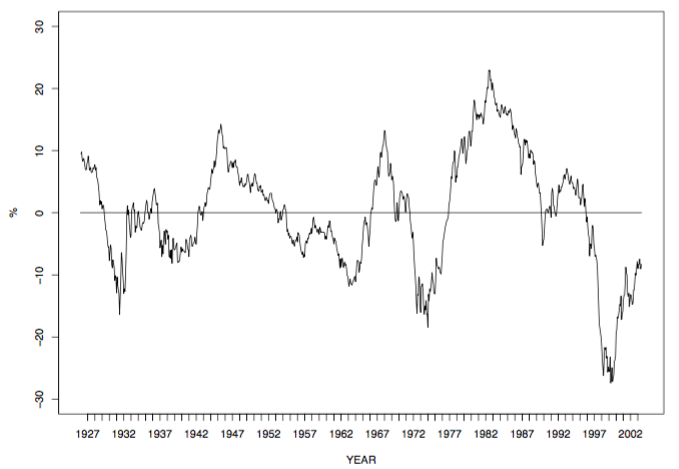
\includegraphics[width=0.9 \linewidth]{CumulativeChangeMarketDiversity}
\caption{Cumulative change in market diversity in the US stock market, 1927--2004, measured by $\pmb{D}_p(\cdot)$, $p=1/2$}
\label{fig:CumChange}
\end{figure}

Note that figure \ref{fig:CumChange} depicts cumulative change due to capital gains and losses, rather than absolute diversity (which is affected by changes in market composition and corporate actions).

\columnbreak

\section{Portfolios of Stocks Selected by Rank}

\subsection{Rank processes and local times}

\paragraph{Rank process $X_{(k)}$}

Let $X_1, \ldots, X_n$ be processes. Then for $k=1, \ldots, n$, the $k$th rank process of $\lbrace X_1, \ldots, X_n \rbrace$ is defined by
\begin{align*}
X_{(k)}(t) = \max\limits_{1 \leq i_1 \leq \ldots \leq i_k \leq n} \min \left( X_{i_1}(t), \ldots, X_{i_k}(t) \right)
\end{align*}

\paragraph{Ranked market weights $\mu_{(k)}$}
\begin{align*}
\mu_{(1)}(t) &\geq \mu_{(2)}(t) \geq \ldots \geq \mu_{(n)}(t) \\
\mu_{(\cdot)} &= \left( \mu_{(1)}(t), \ldots, \mu_{(n)}(t) \right)
\end{align*}
where the $\mu_{(k)}$ are the rank processes associated with the market weights $\mu_1, \ldots, \mu_n$.

\paragraph{Capital distribution of the market}

The ranked family of market weights $\lbrace \mu_{(1)}(t), \ldots, \mu_{(n)}(t) \rbrace$ is the capital distribution of the market at time $t$.

\paragraph{Relative rank covariance processes $\tau_{(ij)}$}

\begin{align*}
\tau_{(ij)}(t) &= \tau_{p_t(i) p_t(j)}(t)
\end{align*}

\paragraph{Local time}

Let $X$ be a continuous semimartingale. Then the local time (at 0) for $X$ is the process $\Lambda_X$ defined for $t \in [0,T]$ by
\begin{align*}
\Lambda_X &= \frac{1}{2} \left( |X(t)| - |X(0)| - \int_0^t \sgn (X(s)) dX(s) \right)
\end{align*}
where $\sgn(x) = 2 \mathbb{I}_{(0,\infty)}(x) - 1$.

Note that if $X$ is an absolutely continuous semimartingale s.t. the set $\lbrace t: X(t) = 0 \rbrace$ has Lebesgue measure 0, then it hold that
\begin{align*}
\Lambda_{|X|}(t) &= 2 \Lambda_X(t), \qquad t \in [0,T], \qquad \text{a.s.}
\end{align*}

\paragraph{Pathwise mutually nondegenerance}

The processes $X_1, \ldots X_n$ are pathwise mutually nondegenerate if:
\begin{enumerate}
\item $\forall i \neq j$, $\lbrace t: X_i(t) = X_j(t) \rbrace$ has Lebesgue measure zero, a.s.;
\item $\forall i<j<k$, $\lbrace t: X_i(t) = X_j(t) = X_k(t) \rbrace = \emptyset$, a.s.
\end{enumerate}

Remarks:
\begin{itemize}
\item Condition (i) states that the paths of two processes $X_i, X_j, i \neq j$ may cross each other but only point-wise.
\item Condition (ii) states that the paths of three processes $X_{i,j,k}$ never cross simultaneously in a single point.
\end{itemize}

\paragraph{Semimartingales}

\begin{itemize}
\item Let $X$ be a continuous semimartingale with decomposition
\begin{align*}
X(t) &= \underbrace{X(0)}\limits_\text{initial value} + \underbrace{M_X(t)}\limits_\text{cont. loc. mart.} + \underbrace{V_X(t)}\limits_\text{cont. process w/ loc. bdd. var.}
\end{align*}
for $t \in [0,T]$, a.s.
\item Then $X$ is absolutely continuous if the random signed measures $dV_X$ and $d\langle X \rangle$ on $[0,T]$ are both a.s. absolutely continuous w.r.t. the Lebesgue measure.
\item Suppose $X$ and $Y$ are absolutely continuous semimartingales. Then the random signed measure $d\langle X,Y \rangle$ is a.s. absolutely continuous w.r.t. the Lebesgue measure on $[0,T]$.
\item Suppose $X_1, \ldots, X_n$ are absolutely continuous semimartingales, and $f$ is a real-valued $C^2$ function defined on the range of $(X_1, \ldots, X_n)$ in $\mathbb{R}^n$. Then $f(X_1, \ldots, X_n)$ is an absolutely continuous semimartingale.
\item Let $X$ and $Y$ be continuous semimartingales with $X$ absolutely continuous, and suppose that the set $\lbrace t: Y(t) = 0 \rbrace$ has Lebesgue measure 0, a.s. Then
\begin{align*}
\int_0^t \mathbb{I}_{\lbrace 0 \rbrace} (Y(s)) dX(s) &= 0, \quad t \in [0,T], \quad \text{a.s.}
\end{align*}
\end{itemize}

\paragraph{Random permutation $p_t$}

Assume $X_1, \ldots, X_n$ to be pathwise mutually nondegenerate absolutely continuous semimartingales.
Then for $t \in [0,T]$, the random permutation $p_t$ of $\lbrace 1, \ldots, n \rbrace$ satisfies for $k = 1, \ldots, n$
\begin{align*}
X_{p_t(k)}(t) &= X_{(k)}(t) \\
p_t(k) < p_t(k+1) &\text{ if } X_{(k)}(t) = X_{(k+1)}(t)
\end{align*}
This applies e.g. to the stock price processes as well as to the market weight processes.

\paragraph{Differential of the rank processes}

Let $X_1, \ldots, X_n$ be pathwise mutually nondegenerate absolutely continuous semimartingales. Then the rank processes $X_{(k)}$ are continuous semimartingales s.t. a.s., for $t \in [0,T]$,
\begin{align*}
dX_{(k)}(t) &= \sum_{i=1}^n \mathbb{I}_{\lbrace i \rbrace} (p_t(k)) dX_i(t) \\
&+ \frac{1}{2} d\Lambda_{X_{(k)} - X_{(k+1)}}(t) - \frac{1}{2} d\Lambda_{X_{(k-1)} - X_{(k)}}(t)
\end{align*}
Remark:
\begin{itemize}
\item The local times only grow when the argument is zero.
\item The local times ensure that $X_{(k-1)} \geq X_{(k)} \geq X_{(k+1)}$.
\end{itemize}

\paragraph{Differential of the market weight processes}

Let $\mathcal{M}$ be a market of stocks $X_1, \ldots, X_n$ that are pathwise mutually nondegenerate. Then the market weight processes $\mu_1, \ldots \mu_n$ satisfy
\begin{align*}
d\log \mu_{(k)}(t) &= \sum_{i=1}^n \mathbb{I}_{\lbrace i \rbrace}(p_t(k)) d\log \mu_i(t) \\
&+ \frac{1}{2} d\Lambda_{\log \mu_{(k)} - \log \mu_{(k+1)}}(t) \\
&- \frac{1}{2} d\Lambda_{\log \mu_{(k-1)} - \log \mu_{(k)}}(t)
\end{align*}

\subsection{Portfolios generated by functions of ranked market weights}

Let $\mathcal{M}$ be market of stocks $X_1, \ldots, X_n$ that are pathwise mutually nondegenerate and let $\pmb{S}$ be a function defined on a neighbourhood $U$ of $\Delta^n$.

\paragraph{Portfolio generating function}

Suppose that there exists a positive $C^2$ function $S$ defined on $U$ s.t. for $(x_1, \ldots, x_n) \in U$,
\begin{align*}
\pmb{S}(x_1, \ldots, x_n) &= S(x_{(1)}, \ldots, x_{(n)})
\end{align*}
and for $i=1, \ldots, n$, $x_i D_i \log S(x)$ is bounded for $x \in \Delta^n$. Then $\pmb{S}$ generates the portfolio $\pi$.

Remark:
\begin{itemize}
\item The generating function $\pmb{S}(\mu(t))$ measures the effect that changes in the capital distribution of the market have on the portfolio $\pi$. \\
This is somewhat different from the previously known generating functions that measured the dependence of the portfolio on individual stocks by name (i.e. index).
\end{itemize}

\paragraph{Portfolio weight process}

\begin{empheq}[box=\widefbox]{align*}
& \frac{\pi_{p_t(k)}(t)}{\mu_{(k)}(t)} = \\
& \qquad D_k \log S(\mu_{(\cdot)}(t)) + 1 - \sum_{j=1}^n \mu_{(j)}(t) D_j \log S(\mu_{(\cdot)}(t))
\end{empheq}

\paragraph{Drift term process}

\begin{empheq}[box=\widefbox]{align*}
& d\Theta(t) = \underbrace{\frac{-1}{2 \pmb{S}(\mu(t))} \sum_{i,j=1}^n D_{ij} S(\mu_{(\cdot)}(t)) \mu_{(i)}(t) \mu_{(j)}(t) \tau_{(ij)}(t) dt}\limits_\text{smooth component} \\
& + \underbrace{\frac{1}{2} \sum_{k=1}^{n-1} \left( \pi_{p_t(k+1)}(t) - \pi_{p_t(k)}(t) \right) d\Lambda_{\log \mu_{(k)} - \log \mu_{(k+1)}}(t)}\limits_\text{local time component}
\end{empheq}

\subsection{Examples of rank-dependent portfolios}

\paragraph{The biggest stock}

\begin{itemize}
\item Let $\pmb{S}(x) = x_{(1)}$.
\item Then: $\pi_{p_t(1)}(t) = 1$ and $\pi_{p_t(k)}(t) = 0$ for $k = 2,\ldots, n$.
\item Drift process: $d\Theta(t) = -\frac{1}{2} d\Lambda_{\log \mu_{(1)} - \log \mu_{(2)}}(t)$
\item Portfolio performance: \\
$d \log \frac{Z_\pi(t)}{Z_\mu(t)} = d \log \mu_{(1)}(t) - \frac{1}{2} d\Lambda_{\log \mu_{(1)} - \log \mu_{(2)}}(t)$
\end{itemize}

Remarks:
\begin{itemize}
\item Since $\mu_{(1)}(t) < 1$ and the local time component of the drift process is decreasing, the long-term relative performance of $\pi$ will suffer if there are many changes of leadership in the market.
\item Accordingly, for the biggest stock to perform well relative to the market, it must: \\
either pay higher than market-average dividends (e.g. ATT before the breakup) \\
or else crush all competitors to allow no changes in market leadership (e.g. Microsoft).
\end{itemize}

\paragraph{The size effect}

\begin{itemize}
\item Let $1<m<n$.
\item Large stock index:
\begin{align*}
\pmb{S}_L(\mu(t)) &= \mu_{(1)}(t) + \ldots + \mu_{(m)}(t) \\
d\log \frac{Z_\xi(t)}{Z_\mu(t)} &= d \log \pmb{S}_L(\mu(t)) \\
& \qquad - \frac{1}{2} \underbrace{\frac{\mu_{(m)}(t)}{\pmb{S}_L(\mu(t))}}\limits_{\xi_{(m)}(t)} d\Lambda_{\log \mu_{(m)} - \log \mu_{(m+1)}}(t)
\end{align*}
\item Small stock index:
\begin{align*}
\pmb{S}_S(\mu(t)) &= \mu_{(m+1)}(t) + \ldots + \mu_{(n)}(t) \\
d\log \frac{Z_\eta(t)}{Z_\mu(t)} &= d \log \pmb{S}_S(\mu(t)) \\
& \qquad + \frac{1}{2} \underbrace{\frac{\mu_{(m+1)}(t)}{\pmb{S}_S(\mu(t))}}\limits_{\eta_{(m+1)}(t)} d\Lambda_{\log \mu_{(m)} - \log \mu_{(m+1)}}(t)
\end{align*}
\item Relative performance:
\begin{align*}
& d\log \frac{Z_\eta(t)}{Z_\xi(t)} = \underbrace{d\log \frac{\pmb{S}_S(\mu(t))}{\pmb{S}_L(\mu(t))}}\limits_\text{change in relative capitalization} \\
& \qquad + \underbrace{\frac{1}{2} \left( \xi_{(m)}(t) + \eta_{(m+1)}(t) \right) d\Lambda_{\log \mu_{(m)} - \log \mu_{(m+1)}}(t)}\limits_\text{drift process}
\end{align*}
\item If the ratio of the relative capitalization of the two indices remains stable over time, then the monotonically increasing drift process determines the relative return.
\item Thus, it is likely that that the return on the small-stock index will eventually be greater than that of the large-stock index.
\item This higher long-term return of the small-stock index is due to the increasing drift process, and the relative level of small-stock risk is irrelevant.
\end{itemize}

\paragraph{Leakage in a diversity-weighted large-stock index}

\begin{itemize}
\item Assumption: Let $\xi$ be a large-stock index generated by $\pmb{S}_L$ and let $\pi$ be a portfolio of stocks held in $\xi$.
\item Then the local time component of $d\log \frac{Z_\pi(t)}{Z_\xi(t)}$ is called leakage.
\item Since $\pi_{(m)}(t) \geq \xi_{(m)}(t)$, leakage is monotonically decreasing.
\item When a capitalization-weighted portfolio is contained in a larger market portfolio, leakage refers to the effect caused by stocks that cross over from the capitalization weighted portfolio to the rest of the market portfolio (i.e. they leak out of the portfolio).
\end{itemize}

\columnbreak

\section{Stable Models of Capital Distribution}

\subsection{Capital distribution curve}

\paragraph{Capital distribution curve} The log-log plot of the market weights arranged in descending order, i.e. the logarithms of the market weights, arranged in descending order, versus the logarithms of their respective ranks:
\begin{align*}
\log k \mapsto \log \mu_{(k)}(t)
\end{align*}
Remarks:
\begin{itemize}
\item As can be seen in figure \ref{fig:CapDistrLogLog}, this log-log plot has exhibited remarkable stability over the decades of the last century.
\item Since the number of stocks contained in the data varies from app. 700 in 1929 to app. 7,500 in 1999, the curve becomes longer the later the period.
\item This linear log-log weight distribution is called a \emph{Pareto distribution}. \\
Although the curves are not exactly straight lines but rather generally concave, the plot suggests an underlying Pareto distribution. \\
The sharply decreasing tails of the distributions may be distorted somewhat, since companies in decline do not immediately leave an exchange.
\item The capital distribution is equivalent to the size distribution of firms, which has been studied extensively.
\item This equity market model is compatible with the observed long-term structure of the capital distribution, but without regard to the mechanism that might have produced that distribution.
\end{itemize}

\begin{figure}[H]
\centering
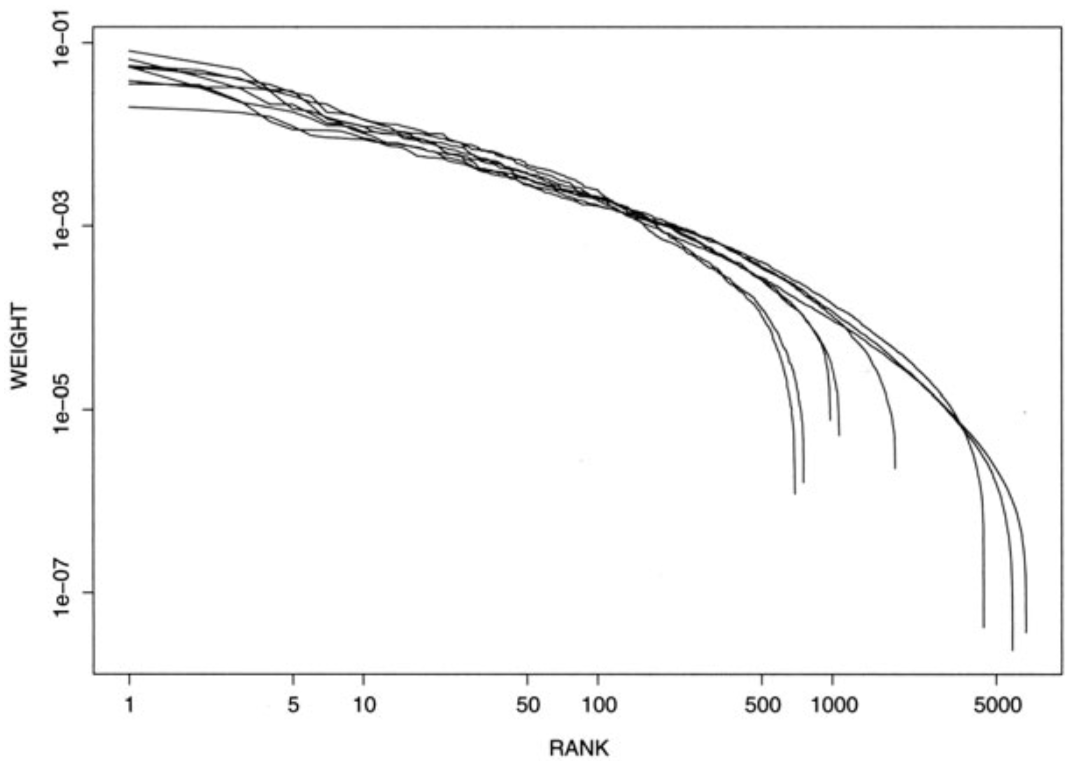
\includegraphics[width=0.8 \linewidth]{CapitalDistributionUS}
\caption{Log-log plot of eight capital distribution curves from the US stock market (1929--1999).}
\label{fig:CapDistrLogLog}
\end{figure}

\paragraph{Capital distribution of the S\&P500}

\begin{itemize}
\item Although the S\&P500 is not the market, it usually holds app. 70\% of the total market capitalization including all of the largest stocks.
\end{itemize}

\begin{figure}[H]
\centering
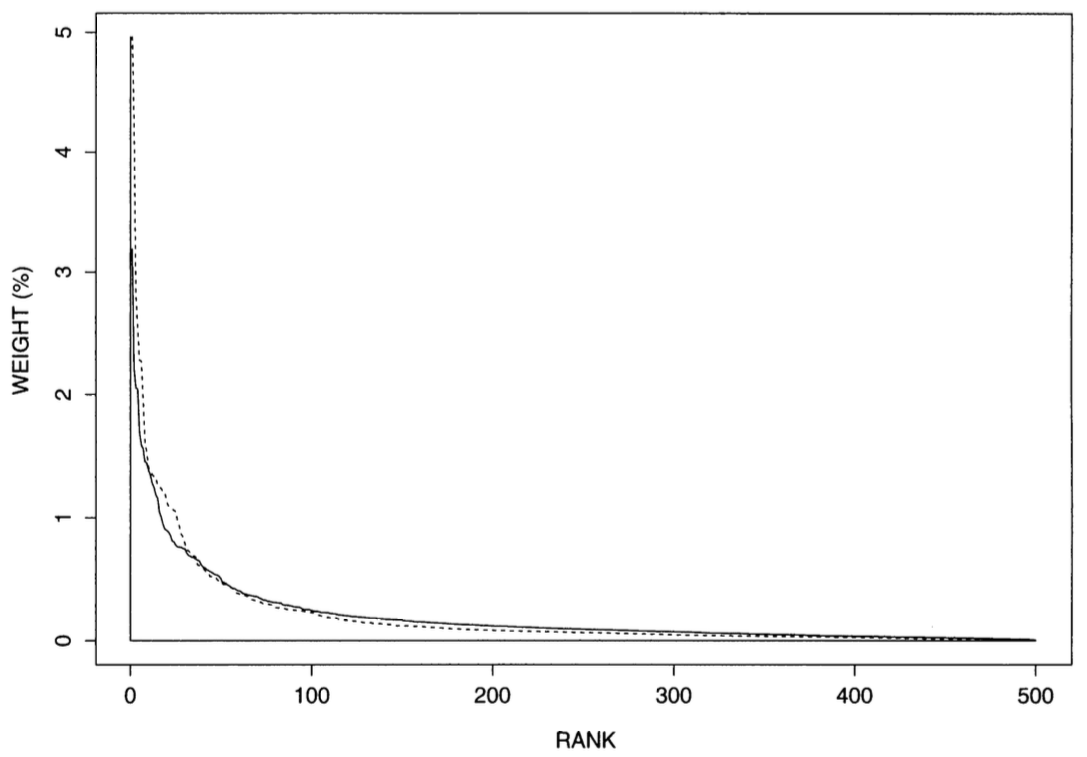
\includegraphics[width=0.8 \linewidth]{CapitalDistributionSPX}
\caption{Linear plot of the capital distribution for the S\&P500 index (1997 (solid line) and 1999 (dotted line)).}
\label{fig:CapDistrLinear}
\end{figure}

\subsection{Structure of stable capital distributions}

\paragraph{Assumptions}

\begin{itemize}
\item Market $\mathcal{M}$ that is coherent and of pairwise mutually nondegenerate stocks $X_1, \ldots, X_n$, along with the corresponding market weights $\mu_1, \ldots, \mu_n$.
\end{itemize}

\paragraph{Asymptotic stability}

The market $\mathcal{M}$ is asymptotically stable if it is coherent and, a.s.
\begin{enumerate}
\item for $k=1, \ldots, n-1$,
\begin{align*}
\lim\limits_{t \to \infty} t^{-1} \Lambda_{\log \mu_{(k)} - \log \mu_{(k+1)}}(t) &= \pmb{\lambda}_{k,k+1}
\end{align*}
\item for $k=1, \ldots, n-1$,
\begin{align*}
\lim\limits_{t \to \infty} t^{-1} \left\langle \log \mu_{(k)} - \log \mu_{(k+1)} \right\rangle_t &= \pmb{\sigma}_{k:k+1}^2
\end{align*}
\end{enumerate}
where $\pmb{\lambda}_{k,k+1}$ and $\pmb{\sigma}_{k:k+1}$ are positive constants. \\
Let $\pmb{\lambda}_{0,1} = 0$ and $\pmb{\lambda}_{n,n+1} = 0$.

Then we say that the capital distribution $\lbrace \mu_{(1)}, \ldots, \mu_{(n)} \rbrace$ is asymptotically stable.

Remarks:
\begin{itemize}
\item Conditions (i) and (ii) imply that asymptotic limits exist for the slopes of the processes $\Lambda_{\log \mu_{(k)} - \log \mu_{(k+1)}}$ and $\left\langle \log \mu_{(k)} - \log \mu_{(k+1)} \right\rangle$.
\end{itemize}

\paragraph{Asymptotic relative growth rate $\pmb{g}_k$}

\begin{itemize}
\item The relative growth rate of $X_{(k)}$ for $k=1,\ldots,n$ is
\begin{align*}
g_k(t) = \gamma_{p_t(k)}(t) - \gamma_\mu(t), \quad t \in [0,\infty)
\end{align*}
\item The asymptotic relative growth rate of $X_{(k)}$, for $k=1, \ldots, n$, is
\begin{align*}
\pmb{g}_k &= \lim\limits_{T \to \infty} \frac{1}{T} \int_0^T g_k(t) dt
\end{align*}
\end{itemize}

\paragraph{Asymptotically stable market}

For the parameters, the following relations hold:
\begin{align*}
\pmb{g}_k &= \frac{1}{2} \pmb{\lambda}_{k-1,k} - \frac{1}{2} \pmb{\lambda}_{k,k+1} \\
\pmb{\lambda}_{k,k+1} &= -2 (\pmb{g}_1 + \ldots + \pmb{g}_k) \\
\pmb{g}_k - \pmb{g}_{k+1} &= \frac{1}{2} \pmb{\lambda}_{k-1,k} - \pmb{\lambda}_{k,k+1} + \frac{1}{2} \pmb{\lambda}_{k+1,k+2}
\end{align*}
Furthermore, it holds that:
\begin{align*}
\pmb{g}_1 + \ldots + \pmb{g}_k &< 0 \\
\pmb{g}_1 + \ldots + \pmb{g}_n &= 0
\end{align*}
Stable model for the log differences between consecutive ranked market weights:
\begin{align*}
& d \left( \log \mu_{(k)}(t) - \log \mu_{(k+1)}(t) \right) = \\
& \qquad - \pmb{\lambda}_{k,k+1}dt + d\Lambda_{\log \mu_{(k)} - \log \mu_{(k+1)}}(t) + dM_{k:k+1}(t)
\end{align*}
where $M_{k:k+1}$ is a continuous martingale with $\langle M_{k:k+1}\rangle_t = \pmb{\sigma}_{k:k+1}^2(t)$.

Remarks:
\begin{itemize}
\item Thus, an asymptotically stable market is characterized by the $2n-2$ \emph{characteristic parameters} $\pmb{g}_1, \ldots, \pmb{g}_{n-1}$ and $\pmb{\sigma}_{1:2}^2, \ldots, \pmb{\sigma}_{n-1:n}^2$.
\item The second equation suggests that for the higher-ranked stocks the $\pmb{g}_k$ are likely to be negative, and for the lower-ranked stocks the $\pmb{g}_k$ are likely to be positive.
\end{itemize}

\paragraph{Slope of the capital distribution curve}

For large enough $k$ it holds a.s.:
\begin{empheq}[box=\widefbox]{align*}
\lim\limits_{T \to \infty} \frac{1}{T} \int_0^T \frac{\log \mu_{(k)}(t) - \log \mu_{(k+1)}(t)}{\log k - \log k+1} dt \approx - \frac{k \pmb{\sigma}_{k:k+1}^2}{2 \pmb{\lambda}_{k,k+1}}
\end{empheq}

\subsubsection{Atlas model}

Let $g$ and $\sigma$ be positive constants and suppose we have stocks $X_1, \ldots, X_n$ that satisfy
\begin{align*}
d \log X_i(t) &= \gamma_i(t) dt + \sigma dW_i(t)
\end{align*}
where
\begin{align*}
\gamma_i(t) &=
\begin{cases}
ng & : X_i(t) = X_{(n)}(t) \\
0 & \text{otherwise}
\end{cases}
= n g \mathbb{I}_{\lbrace 0 \rbrace} \left( X_i(t) - X_{(n)}(t) \right)
\end{align*}

\begin{itemize}
\item The market of the Atlas model is coherent.
\item The Atlas model has the characteristic parameters $\pmb{g}_1 = \ldots = \pmb{g}_{n-1} = -g$ and $\pmb{\sigma}_{1:2}^2 = \ldots = \pmb{\sigma}_{n-1:n}^2 = 2 \sigma^2$. \\
It follows that $\pmb{g}_n = (n-1)g$. \\
Furthermore, it holds that $\pmb{\lambda}_{k,k+1} = 2kg$ for $k = 1=1,\ldots,n-1$.
\item The log-log slope between $\mu_{(k)}$ and $\mu_{(k+1)}$ is the constant $-\sigma^2/2g$, so the asymptotic capital distribution follows a Pareto distribution.
\item Since it holds a.s.
\begin{align*}
\lim_{T \to \infty} \frac{1}{T} \int_0^T \log X_{(k)}(t) = \lim_{T \to \infty} \frac{1}{T} \int_0^T \gamma_\mu(t) dt = g
\end{align*}
the whole market should asymptotically grow at the rate $g$. \\
This is reasonable since the smallest stock has growth rate $ng$ and the other stocks have growth rate zero, and each stock is smallest about $1/n$ of the time.
\end{itemize}

\subsection{Application to the US equity market}

\begin{figure}[H]
\centering
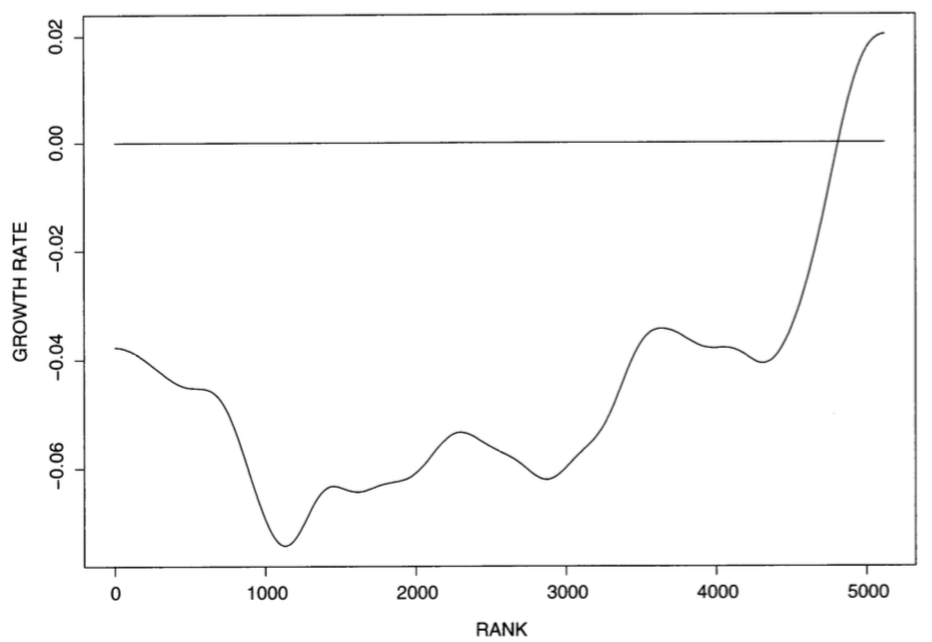
\includegraphics[width=0.8 \linewidth]{USGrowthRates}
\caption{Smoothed annualized values of $\pmb{g}_k$ for $k=1, \ldots, 5119$, based on data from 1990 to 1999.}
\label{fig:USGrowthRates}
\end{figure}

\begin{itemize}
\item The values of the $\pmb{g}_k$ as shown in figure \ref{fig:USGrowthRates} go from negative for the larger stocks to positive for the smallest stocks.
\item This curve shows considerable structure, which might not be stable over time.
\end{itemize}

\begin{figure}[H]
\centering
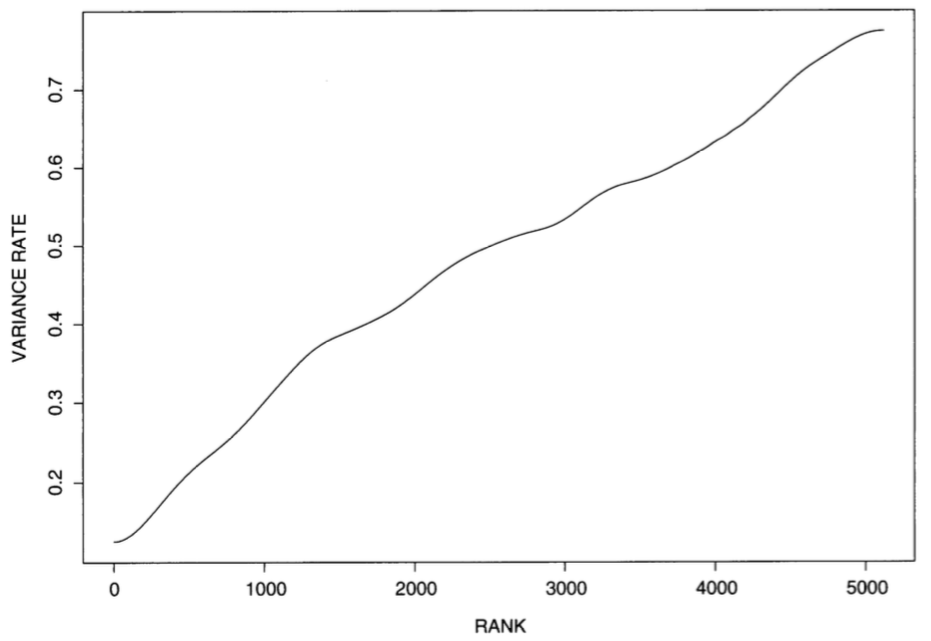
\includegraphics[width=0.8 \linewidth]{USVariances}
\caption{Smoothed annualized values of $\pmb{\sigma}_{k:k+1}^2$ for $k=1, \ldots, 5119$, based on data from 1990 to 1999.}
\label{fig:USVariances}
\end{figure}

\begin{itemize}
\item The values of the $\pmb{\sigma}_{k:k+1}^2$ as shown in figure \ref{fig:USVariances} form an increasing, approximately straight line.
\item It appears that between the largest stocks, the relative annual standard deviation is app. 35\%, while between the smallest stocks it is app. 85\%.
\end{itemize}

\subsection{First-order model}

\begin{itemize}
\item This is a simple first-order approximation to a market model that is compatible with the $2n-2$ structural parameters defined for the stable capital distribution.
\item The growth rates $\pmb{g}_k$ will be used without modification and $\pmb{g}_k$ will be the growth rate of the $k$th-ranked stock $X_{(k)}$.
\item The $\pmb{\sigma}_{k:k+1}^2$ represent variance parameters for the differences of the logarithmic returns of consecutively ranked stocks. \\
It is assumed that the stock processes are independent, i.e. that there is no cross-variation of the stock processes to be considered (since the $\pmb{\sigma}_{k:k+1}^2$ contain little if any information about the cross-variation of the stock processes).
\end{itemize}

\paragraph{Definition}

\begin{itemize}
\item Suppose that the market $\mathcal{M}$ has an asymptotically stable capital distribution.
\item $\pmb{g}_k$ and $\pmb{\sigma}_{k:k+1}^2$, for $k=1,\ldots,n-1$ are the characteristic parameters of the distribution.
\item Under the assumption that the ranked stocks are independent (i.e. there is no cross-variation), it holds for the variation that
\begin{align*}
\pmb{\sigma}_{k:k+1}^2 &= \pmb{\sigma}_k^2 + \pmb{\sigma}_{k+1}^2
\end{align*}
\item For the variation, it holds that
\begin{align*}
\pmb{\sigma}_k^2 &= \frac{1}{4} \left( \pmb{\sigma}_{k-1:k}^2 + \pmb{\sigma}_{k:k+1}^2 \right) & \text{for } k = 2, \ldots, n-1 \\
\pmb{\sigma}_1^2 &= \frac{1}{2} \pmb{\sigma}_{1:2}^2 \qquad \pmb{\sigma}_n^2 = \frac{1}{2} \pmb{\sigma}_{n-1:n}^2
\end{align*}
\item With $q_t$ being the inverse of the permuation $p_t$, the first-order model is given by:
\begin{empheq}[box=\widefbox]{align*}
d\log X_i(t) &= \pmb{g}_{q_t(i)} dt + \pmb{\sigma}_{q_t(i)} dV_i(t)
\end{empheq}
for $i=1,\ldots,n$, where $(V_1,\ldots,V_n)$ is an $n$-dimensional BM.
\end{itemize}

Remarks:
\begin{itemize}
\item Obviously, the first-order market model is much simpler than the general market model for it depends on $2n-2$ constant parameters rather than $n^2+n$ stochastic processes.
\item Empirical data suggests that the structural parameters $\pmb{g}_k$ and $\pmb{\sigma}_{k:k+1}^2$ vary somewhat over time, and that this variation causes the spread in the actual curves that is not present in the simulated curves.
\item The variation of the diversity of the actual market is greater than the variation of the diversity of a simulated market by the first-order model.
\end{itemize}

\columnbreak
%\newpage

\section{Appendix}

\paragraph{Symmetric function}

A real-valued function $F$ defined on a subset of $\mathbb{R}^n$ is symmetric if it is invariant under permutations of the variables $x_i, i = 1, \ldots, n$.

\paragraph{Concave function}

A real-valued function $F$ defined on a subset of $\mathbb{R}^n$ is concave if for $0<p<1$ and $x,y \in \mathbb{R}^n$ it holds that
\begin{align*}
F(p x + (1-p) y) > p (F(x) + (1-p) F(y).
\end{align*}

\paragraph{Simplex}

The simplex is defined as the following set:
\begin{align*}
\Delta^n = \lbrace x \in \mathbb{R}^n : x_1 + \ldots + x_n = 1 ; 0 < x_i < 1 , i = 1, \ldots, n \rbrace
\end{align*}

\paragraph{Notation of partial derivatives}

\begin{itemize}
\item $D_i$ denotes the partial derivative w.r.t. the $i$th variable.
\item $D_{i j}$ denotes the second partial derivative w.r.t. the $i$th and $j$th variables.
\end{itemize}

\paragraph{Continuous semimartingale}

A continuous semimartingale $X$ is a measurable, adapted process that has the decomposition
\begin{align*}
X(t) = X(0) + M_X(t) + M_X(t) + V_X(t), \qquad t \in [0,\infty)
\end{align*}
where $M_X$ is a continuous, square-integrable local martingale and $V_X$ is a continuous, adapted rpcoess of bounded variation.

The \emph{cross-variation process} of two semimartingales is defined as
\begin{align*}
\langle X,Y \rangle = \langle M_X,M_Y \rangle
\end{align*}
where $M_X$ and $M_Y$ are the local martingale parts of $X$ and $Y$, respectively.

The quadratic variation process for $X$ is similarly defined as $\langle X \rangle = \langle M_X \rangle$.

\paragraph{Cross-variation of standard Brownian motion}

\begin{align*}
\langle W_i,W_j \rangle_t = \delta_{ij}, \qquad t \in [0,\infty)
\end{align*}
where $\delta_{ij} = 1$ if $i=j$, and $0$ otherwise.

\columnbreak
\begin{center}
\textit{intentionally left blank}
\end{center}
\vfill

\section*{Abbreviations}

\begin{description}[style=multiline,leftmargin=1cm,font=\textbf]
\item[a.s.] almost surely
\item[BM] Brownian motion
\item[EMM] equivalent martingale measure
\item[IOT] in order to
\item[mart.] martingale
\item[PDE] partial differential equation
\item[RV] random variable
\item[SDE] stochastic differential equation
\item[SPT] stochastic portfolio theory
\item[s.t.] such that
\item[w.l.o.g.] without loss of generality
\item[w.r.t.] with respect to
\end{description}

\section*{Disclaimer}

\begin{itemize}
\item This summary is work in progress, i.e. neither completeness nor correctness of the content are guaranteed by the author.
\item This summary may be extended or modified at the discretion of the readers.
\item Source: Lecture New Trends in Stochastic Portfolio Theory, autumn semester 2015/16, ETHZ (lecture notes and corresponding book). Copyright of the content is with the lecturers.
\item The layout of this summary is mainly based on the summaries of several courses of the BSc ETH ME from Jonas LIECHTI.
\end{itemize}

\end{multicols*}

\end{document}